\documentclass[10pt]{beamer}
\usetheme{CambridgeUS}
\usecolortheme{beaver}
\usepackage{shortcut2}

% Title page details
\title{Distributional Reinforcement Learning and Quantile Optimization}
\subtitle{Internship Oral Defense}
\author{Alexandre Marthe}
\institute{ENS de Lyon}
\date{\today}

\begin{document}

\AtBeginSection[]
{
  \begin{frame}
    \frametitle{Table of Contents}
    \tableofcontents[currentsection]
  \end{frame}
}

\begin{frame}
% Print the title page as the first slide
\titlepage
\end{frame}

\begin{frame}
    \begin{figure}
        \centering
            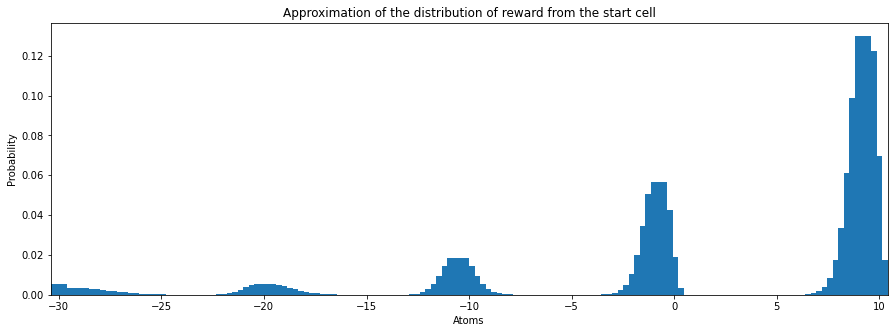
\includegraphics[width=0.8\textwidth]{figures/personal_work/distrib_q80.png}
        \caption{Example of distribution where the mean gives little information}
    \end{figure}
\end{frame}

\begin{frame}{Table of Contents}
    \tableofcontents
\end{frame}

\section{The general RL framework}
\begin{frame}{Markov Decision Process\cite{szepesvari2010algorithms}}
    \begin{definition}[Markov Decision Processes]
        An MPD is a tuple $\MM(\XX, \AAA, P, \gamma)$, where:
        \begin{itemize}
            \item $\XX$ is a finite state space
            \item $\AAA$ a finite action space
            \item $P$ a transition probability kernel that assigns to each pair $(x,a) \in \XX \times \AAA$ a probability measure on $\XX \times \RR$
            \item $\gamma \in [0,1[$ the discount
        \end{itemize}
        
        \end{definition}
        The \emph{return}, that we aim to optimize is:
        \[ R = \EE{ r(x_0, a_0) + \gamma r(x_1, a_1) + \gamma^2 r(x_2, a_2) +  \dots} = \EE{\sum_{t=0}^\infty  \gamma^t r(x_t, a_t)} \]
\end{frame}

\begin{frame}
    \begin{definition}
        A decisision rule $d$ is a function that maps each state to a probability distribution on the action space :
        
        \[ d: \XX \mapsto \PPPP(\AAA) \]
    
        It is said \emph{deterministic} if it of the form d: $\XX \mapsto \AAA$ \\
    \end{definition}
    
    \begin{definition}
        A policy is a sequence of decision rule: 
    
        \[ \pi = (d_0, d_1, d_2, \dots) \]
    
        It is said \emph{stationnary} if it uses a unique decision rule.
    \end{definition}
\end{frame}

\begin{frame}
    \begin{theorem}[Bertsekas, 2007]
        If an optimal policy exists, it can be chosen to be stationnary.
    \end{theorem}
    \begin{proposition}[Bellman optimality principle\cite{bellman1966dynamic}]
        An optimal policy has the property that whatever the initial state and initial decision are, the remaining decisions must constitute an optimal policy with regard to the state resulting from the first decision.
    \end{proposition}
    
    \begin{corollary}
        If an optimal policy exists, then it can be chosen to be deterministic.
    \end{corollary}       
\end{frame}

\begin{frame}
    \begin{definition}
        The Value functions $V$ and $Q$ are defined by:
        \begin{align*}
            V^\pi(x) &= \EE{\sum_{t=0}^\infty  \gamma^t r(x_t, a_t) | x_0 = x} \\
            Q^\pi(x,a) &= \EE{\sum_{t=0}^\infty  \gamma^t r(x_t, a_t) | x_0 = x, a_0 = a}
        \end{align*}
        with $x_t \sim p(\cdot | x_{t-1}, a_{t-1})$ and $a_t \sim \pi(\cdot | x_t)$
    \end{definition}

    \begin{definition}
        The Optimal Value functions $\sta V$ and $\sta Q$ are defined by:
        \begin{align*}
            \sta V(x) &= \max_{\pi} \EE{\sum_{t=0}^\infty  \gamma^t r(x_t, a_t) | x_0 = x} = V^{\sta\pi}(x)\\
            \sta Q(x,a) &= \max_{\pi} \EE{\sum_{t=0}^\infty  \gamma^t r(x_t, a_t) | x_0 = x, a_0 = a} = Q^{\sta\pi} (x,a)
        \end{align*}
    \end{definition}
\end{frame}

\begin{frame}
    \begin{definition}[Bellman Operator]
        Let $V: \XX \mapsto \RR$ or $Q: \XX \times \AAA \mapsto \RR$, $\pi$ a policy. The Bellman operator $\TT^\pi$ is defined by:
        \[ \forall x \in \XX, \qquad \TT^\pi V(x) = \sum_{a \in \AAA} \pi(a|x) \left( \EE{r(x,a)} + \gamma \sum_{x^\prime  \in \XX} p(x^\prime |x,a)V(x^\prime ) \right) \]
        \[ \forall x,a \in \XX \times \AAA, \qquad \TT^\pi Q(x,a) = \EE{r(x,a)} + \gamma \sum_{x^\prime ,a^\prime  \in \XX \times \AAA} p(x^\prime |x,a)\pi(a^\prime |x^\prime )Q(x^\prime ,a^\prime ) \]
    \end{definition}
    \begin{definition}[Optimal Bellman Operator]
        Let $V: \XX \mapsto \RR$ or $Q: \XX \times \AAA \mapsto \RR$, $\pi$ a policy. The Bellman operator $\sta \TT$ is defined by:
        \[ \forall x \in \XX, \qquad \sta\TT V(x) = \max_{a \in \AAA} \EE{r(x,a)} + \gamma \sum_{x^\prime  \in \XX} p(x^\prime |x,a)\sta V(x^\prime ) \]
        \[ \forall x,a \in \XX \times \AAA, \qquad \sta \TT Q(x,a) = \EE{r(x,a)} + \gamma \sum_{x^\prime  \in \XX} p(x^\prime |x,a)\max_{a^\prime  \in \AAA}\sta Q(x^\prime ,a^\prime ) \]
    \end{definition}
\end{frame}

\begin{frame}
    \begin{proposition}
        The Bellman Operators are $\gamma$-contractions.
    \end{proposition}

    \begin{theorem}[Banach fixed point\cite{rudin1991functional}]
        Let $( X , d )$ be a non-empty complete metric space with a contraction mapping $ T : X \mapsto X$. Then $T$ has admits a unique fixed-point $\sta x\in X$ and
        \[ \forall x \in X, \quad T^n(x) \longrightarrow \sta x \text{ exponentially} \]
    \end{theorem}

    \begin{corollary}[Algorithms]
        Iterating the Bellman operators is an algorithm to compute the value functions.
    \end{corollary}
\end{frame}
































\section{The Distributional RL framework}


\subsection*{Metrics}
\begin{frame}{Metrics}
    \begin{definition}[Wasserstein Metric\cite{rowland_analysis_2018}]
        Let $p \geq 1$ and $\PPPP_p(\RR)$ the space of distributions with finite $p^{\text{th}}$ moment. Let $\nu_1, \nu_2 \in \PPPP_p(\RR)$  with respective cumulative distribution function $F$ and $G$. The p-Wasserstein distance $d_p$ is then defined as :
    
        \[ d_p(\nu_1, \nu_2) = \left(\int_0^1\left|F^{-1}(u) - G^{-1}(u)\right|^p du\right)^{\frac{1}{p}} \]
    \end{definition}
    \begin{definition}[\cite{rowland_analysis_2018}]
        Let $\nu_1, \nu_2 \in \PPPP(\RR)$. We define the family of metrics $\ell_p$ by :
    
        \[ \ell_p(\nu_1, \nu_2) = \left( \int_\RR (F_{\nu_1}(x) - F_{\nu_2}(x))^p \dd x\right)^{\frac{1}{p}} \]
    
        $\ell_2$ is called the Cramer distance.
    \end{definition}
\end{frame}

\begin{frame}{Framework}
    The random return is the sum of the discounted random reward:

    \begin{equation}
        Z(x,a) = \sum_{t = 0}^{\infty} \gamma R_t \ |\ X_0 = x, A_0 = a
    \end{equation}
    
    The idea is that the distribution of the reward would follow similar Bellman equations:
    
    \begin{equation}\label{randvarbellman}
        Z(x,a) \deq R(x,a) + \gamma Z(X^\prime, A^\prime)
    \end{equation}
    
    with $X^\prime, A^\prime$ the random next state-action.
\end{frame}


\subsection*{Policy Evaluation}
\begin{frame}{Policy Evaluation}
    Let’s consider a policy $\pi$. The distribution of the random return under $\pi$ will be written as follows:

    \[ \eta_\pi^{(x,a)} = \text{Law}_\pi \left( \sum_{t = 0}^{\infty} \gamma R_t \ | \ X_0 = x, A_0 = a \right) \]

    The random return associated to policy $\pi$ verifies the \emph{distributional Bellman equation}:
    \[\eta_\pi = \TT^\pi \eta_\pi \]
    where $\TT^\pi$ is the Bellman operator defined by:
    
    \[
        \TT^\pi \eta^{(x,a)} = \int_\RR \sum_{(x^\prime,a^\prime)\in \XX \times \AAA} (f_{r,\gamma})_\#\eta^{(x^\prime,a^\prime)}\pi(a^\prime|x^\prime)p(r,x^\prime|x,a)dr
    \]

    with $(f_{r,\gamma})_\#\eta$ is the pushforward measure define by $f_\#\eta(A) = \eta(f^{-1}(A))$ for all Borel sets $A\subseteq R$ and $f_{r,\gamma}(x) = r + \gamma x$ for all $x \in R$.
\end{frame}

\begin{frame}
    \begin{proposition}
        $\TT^\pi$ is a $\gamma$-contraction under the maximal $p$-Wasserstein metric $\overline{d}_p$ (for $p \geq 1$).
    \end{proposition}
    \begin{corollary}
        \[ \forall \eta \in \PPPP(\RR)^{\XX \times \AAA}, \quad (\TT^\pi )^n \eta \underset{n \rightarrow \infty}{\longrightarrow} \eta_\pi \]
        with an exponential convergence for the norm $\overline{d}_p$.
    \end{corollary}
\end{frame}

\subsection*{Control}
\begin{frame}{Control}
    We define by optimal distribution a distribution associated to an optimal policy: 

\[    \sta\eta \in \{ \eta_{\sta\pi} \ | \ \sta\pi \in \argmax_{\pi} \EEE{R \sim \eta_\pi}{R}\}
\]

    As expected, the optimal distributions verify the optimal distributional Bellman equation: $\sta\eta = \TT\sta\eta$ with 

\[
    \TT\eta^{(x,a)} = \int_\RR \sum_{(x^\prime,a^\prime)\in \XX \times \AAA} (f_{r,\gamma})_\#\eta^{(x^\prime,\sta a(x^\prime))}p(r,x^\prime|x,a)dr
\]
where $\sta a(x^\prime) = \argmax_{a^\prime \in \AAA} \EEE{R \sim \eta^{(x^\prime, a^\prime)}}{R}$
\end{frame}

\begin{frame}
    \begin{lemma}
        Let $\eta_1, \eta_2 \in \PPPP(\RR)^{\XX\times\AAA}$, we write $\EE{\eta}:= \EEE{Z \sim \eta}{Z}$. Then:
        \[ \norm{\EE{\TT\eta_1} - \EE{\TT\eta_2}}_\infty \leq \gamma \norm{\EE{\eta_1} - \EE{\eta_2}}_\infty \]  
    
        Which means that $\EE{\TT^n \eta} \underset{n \rightarrow \infty}{\longrightarrow} \sta Q$ exponentially quickly.
    \end{lemma}
    
    But also:

    \begin{theorem}
        Let $\XX$ and $\AAA$ be finite. Let $\eta \in \PPPP(\RR)^{\XX\times\AAA}$. There exist an optimal policy $\sta \pi$ (potentially nonstationary), such that: 
        
        \[\TT^n \eta \underset{n \rightarrow \infty}{\longrightarrow} \eta_{\sta \pi} \text{ uniformly in } \overline{d}_p, \ p\geq1\]
    \end{theorem}
\end{frame}

\begin{frame}
    \begin{proposition}
        The optimality operators are not always contractions.
    \end{proposition}
    
    \begin{proposition}
        The optimality operators do not always have fixed points.
    \end{proposition}
\end{frame}

\subsection*{Distribution approximations}
\begin{frame}{Distribution approximations}
    Main issue: we need a way to approximate the distributions. We have parametrizations:
    \begin{itemize}
        \item Categorical Parametrization
        \item Quantile Parametrization
    \end{itemize}
\end{frame}

\begin{frame}{Categorical Approach}
    The idea is to use the hypothesis of bounded reward to use evenly spread diracs on that reward support, and use the diracs weight as the parameters.

\begin{figure}[!ht]
    \centering
    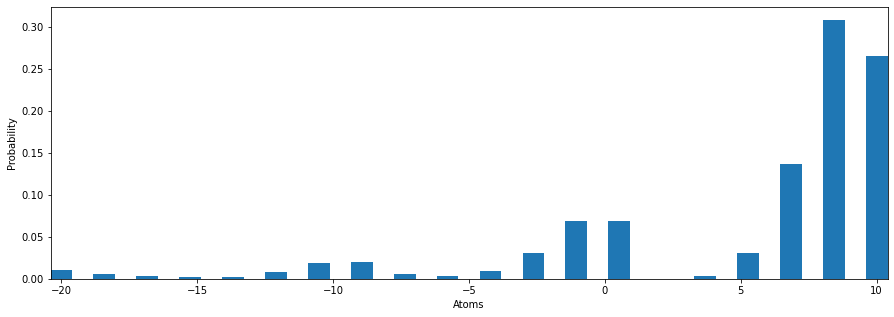
\includegraphics[height=0.35\textheight]{figures/personal_work/categoriacl.png}
    \caption{Example of a distribution projected by with the categorical approach}
\end{figure}

    The projection operator is defined by: \begin{equation}
        \Pi_C(\delta_y) = 
        \begin{cases}
            \delta_{z_0} & y \leq z_0\\
            \frac{z_{i+1}-y}{z_{i+1}-z_{i}}\delta_{z_i} + \frac{y - z_i}{z_{i+1}-z_{i}}\delta_{i+1} & z_i < y < z_{i+1}\\
            \delta_{z_{N-1}} & y \geq z_{N-1}
        \end{cases}
    \end{equation}
\end{frame}

\begin{frame}
    \begin{proposition}
        $\Pi_C\TT^\pi$ is not a contraction for $\overline{d}_p$ with $p > 1$.
    \end{proposition}
    \begin{proposition}
        $\Pi_C\TT^\pi$ is a $\sqrt[p]\gamma$-contraction in $\overline{\ell}_p$.
    \end{proposition}
    \begin{equation}\label{ProjBellmanCatConv}
        \exists ! \eta_C \in \PPP_C^{\XX \times \AAA}, \ \forall \eta_0 \in \PPPP(\RR)^{\XX \times \AAA},\quad (\Pi_C\TT^\pi)^m\eta_0 \underset{m \rightarrow \infty}{\longrightarrow} \eta_C \quad \text{exponentially quickly in } \overline{\ell}_p
    \end{equation}
    \begin{lemma}
        Let $\eta_C$ defined as in (\ref{ProjBellmanCatConv}). Assume that $\eta_\pi$ is supported on $[z_0, z_{N-1}]$. Then:
        \[ \overline{\ell}_2(\eta_C, \eta_\pi) \leq \frac{1}{1-\gamma} \Delta z \]
    \end{lemma}
\end{frame}

\begin{frame}{Quantile Approach}
    We define the quantile projection operator by $\displaystyle \Pi_{d_1}\nu = \frac{1}{N} \sum_{i = 0}^{N-1} \delta_{z_i}$ with $\displaystyle z_i = F^{-1}\left(\frac{2i + 1}{2N}\right)$. This leads to a minization of the Wasserstein metrics between the true distribution and the parametrized space.

    \begin{figure}[!ht]
        \centering
        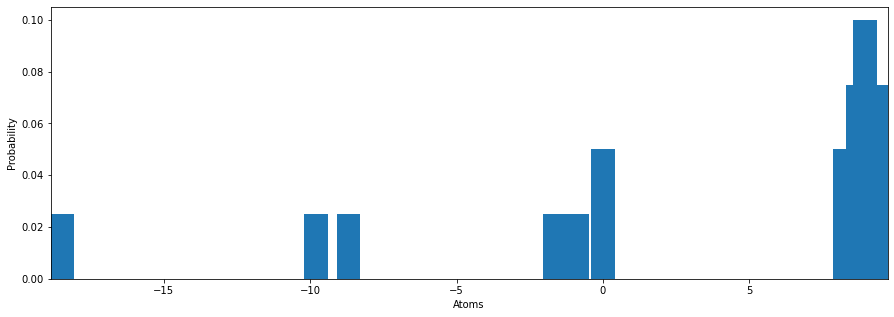
\includegraphics[height=0.4\textheight]{figures/personal_work/quantile.png}
        \caption{Example of a distribution projected with the quantile approach}
    \end{figure}
\end{frame}

\begin{frame}
    \begin{proposition}
        $\Pi_{d_1}\TT^\pi$ is $\gamma$-contraction in $\overline{d}_\infty$ :
    
        \[ \overline{d}_\infty(\Pi_{d_1}\TT^\pi\eta_1 , \Pi_{d_1}\TT^\pi\eta_2) \leq \gamma \overline{d}_\infty(\eta_1, \eta_2)\]
    \end{proposition}
\end{frame}

























\section{Personnal Work}
\begin{frame}{Framework}
    We are still considering MDPs of the form $\MM(\XX,\AAA, P,R, \gamma)$, but with another value to optimize. We consider $x \in \XX$ a specific state, and $\tau \in [0,1]$ the quantile of interest. Our objective is:

\[\max_\pi V_\tau(x) = q_\tau\left(\sum_{t = 0}^{\infty} \gamma R_t \ |\ X_0 = x\right) \]
\end{frame}

\begin{frame}{Cliff environment}
    \begin{figure}[!ht]
        \centering
    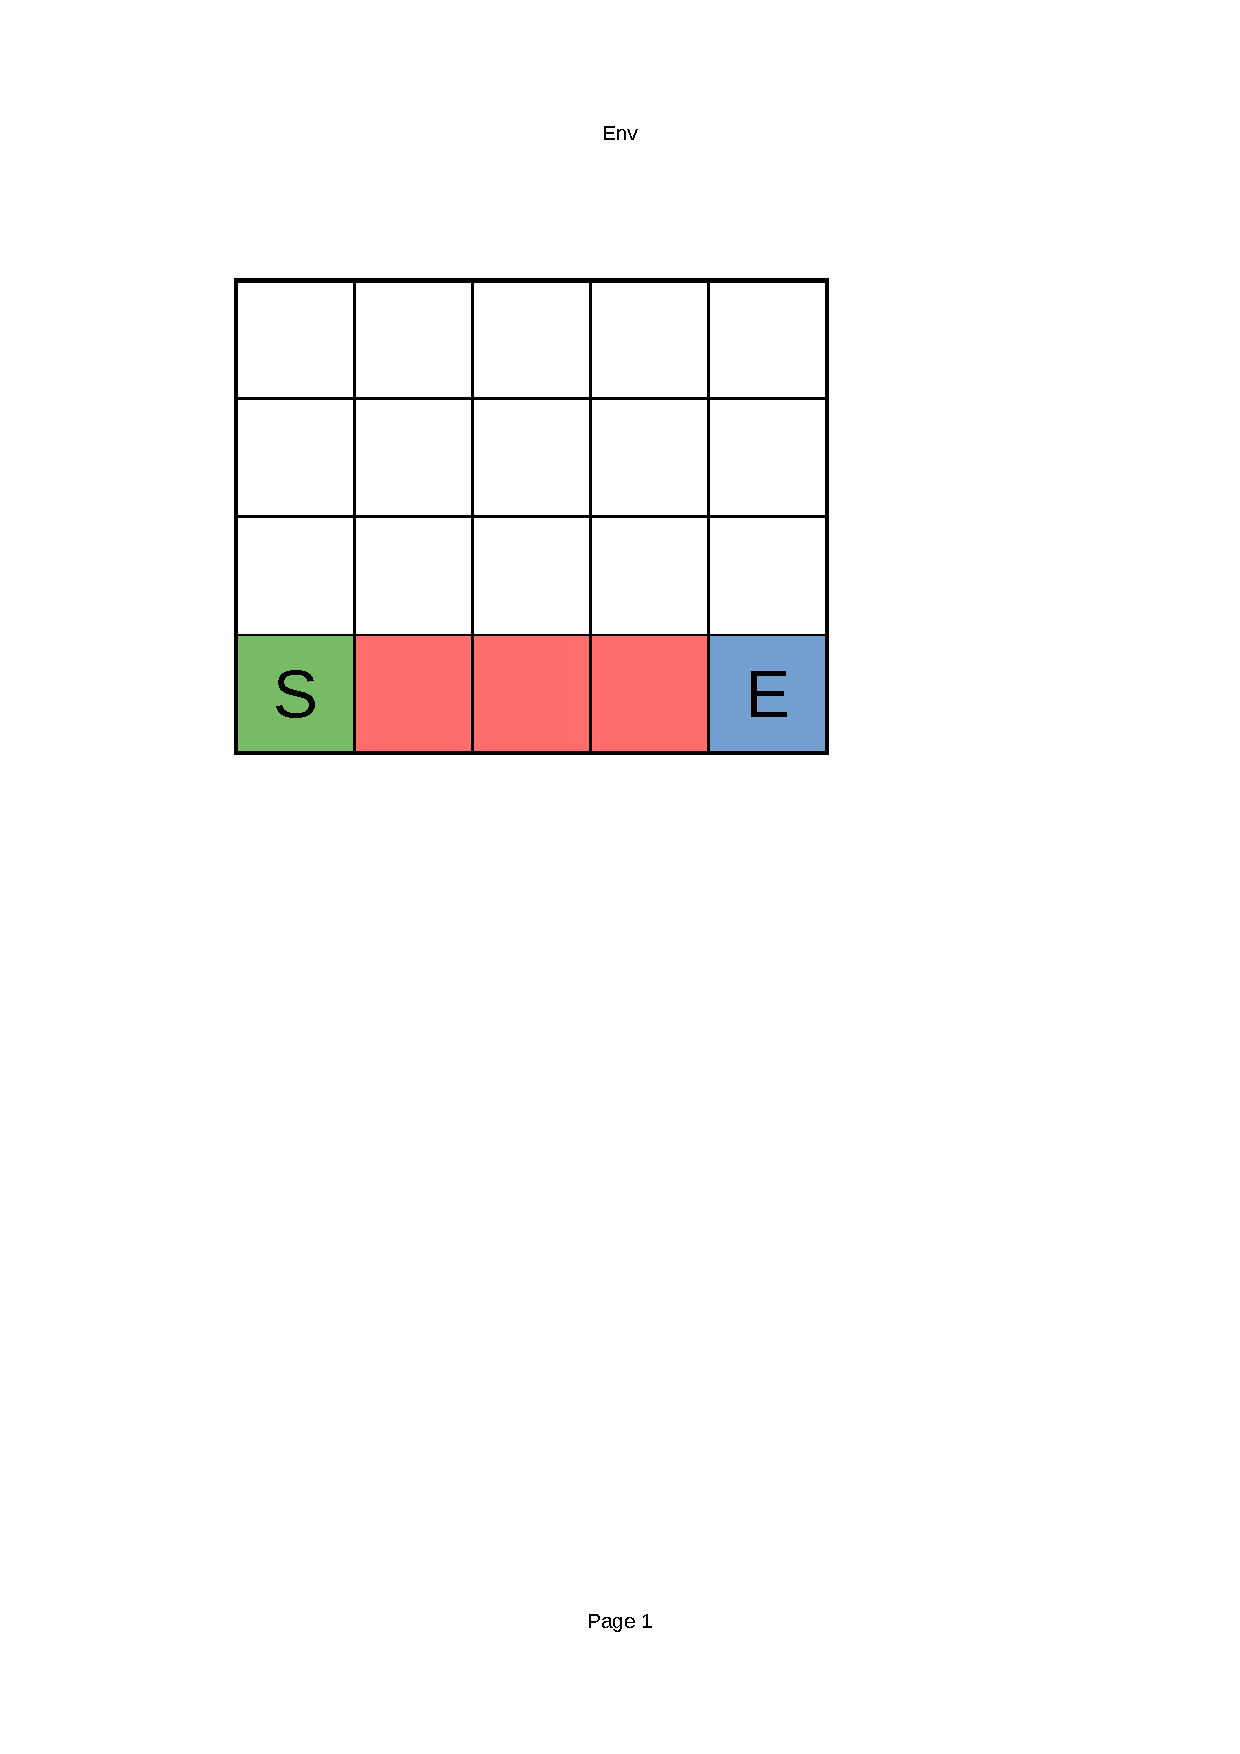
\includegraphics[page=1, trim = 40mm 160mm 70mm 45mm, clip, height=0.4\textheight]{figures/personal_work/policies.pdf}
    \caption{State space of the Cliff environment}
    \end{figure}

    The reward received when reaching E is set to $10$. The reward received when falling is set to $-10$.

    The agent can move in the $4$ directions, but has only $0.7\%$ chances to go in the chosen direction, and has $0.1\%$ chances to go any other direction.
\end{frame}

\subsection*{Policy Evaluation}
\begin{frame}{Policy Evaluation}
    In Practice:
    \begin{itemize}
        \item Iterating the Bellman algorithm and compute the quantile of the output distribution works well
    \end{itemize}

    \bigskip

    In Theory:
    \begin{itemize}
        \item No guaranteed bound on the difference between the computed quantile and the real one.
    \end{itemize}

    \[ (\TT^\pi )^n \eta \underset{n \rightarrow \infty}{\longrightarrow} \eta_\pi \quad \nRightarrow \quad q_\tau\left((\TT^\pi )^n \eta\right) \underset{n \rightarrow \infty}{\longrightarrow} q_\tau(\eta_\pi)  \]

\end{frame}

\begin{frame}
    \begin{figure}[!ht]
        \centering
        \begin{subfigure}{0.25\textwidth}
            \centering
                \includegraphics[page=2, trim = 40mm 160mm 70mm 45mm, clip, width=0.95\textwidth]{figures/personal_work/policies.pdf}
            \caption{Safe policy}
        \end{subfigure}
        \hfill
        \begin{subfigure}{0.70  \textwidth}
            \centering
                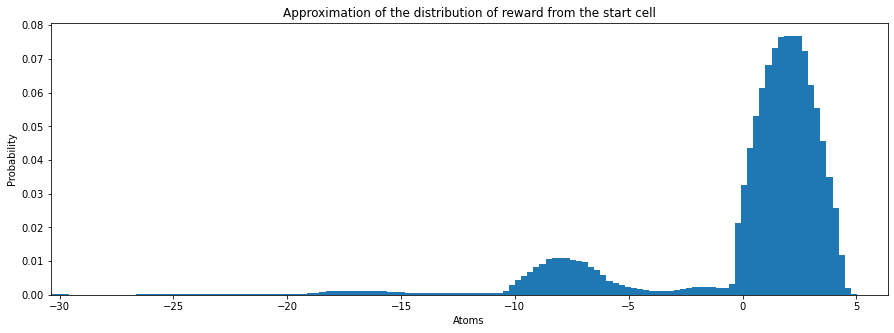
\includegraphics[ width=\textwidth]{figures/personal_work/distrib_safe_policy2.png}
            \caption{Distribution of return}
        \end{subfigure}
    \end{figure}
    
    \begin{figure}[!ht]
        \centering
        \begin{subfigure}{0.25\textwidth}
            \centering
                \includegraphics[page=3, trim = 40mm 160mm 70mm 45mm, clip, width=0.95\textwidth]{figures/personal_work/policies.pdf}
            \caption{Risky policy}
        \end{subfigure}
        \hfill
        \begin{subfigure}{0.70\textwidth}
            \centering
                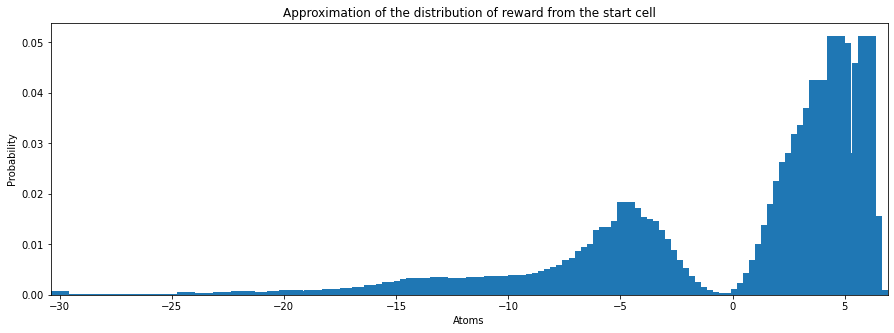
\includegraphics[ width=\textwidth]{figures/personal_work/distrib_greedy_policy.png}
            \caption{Distribution of return}
        \end{subfigure}
    \end{figure}
\end{frame}

\subsection*{Control}
\begin{frame}{Counter example Bellman Optimality Principle}
    \begin{center}
        \begin{tikzpicture} [node distance = 3cm, on grid, auto]
            \node (q1) [state] {$q_1$};
            \node (q2) [state, above left = of q1] {$q_2$};
            \node (q3) [state, above right = of q1] {$q_3$};
            \node (q4) [state, above left = of q3] {$q_4$};
            \node (q5) [state, above right = of q3] {$q_5$};
    
            \path [-stealth, thick]
        (q1) edge node {p = 0.7, r=10}   (q2)
        (q1) edge node {p = 0.3, r=0}   (q3)
        (q3) edge node {2, 3}   (q4)
        (q3) edge node {1, 4}   (q5);    
        \end{tikzpicture}
    \end{center}
\end{frame}

\begin{frame}
    \begin{figure}[!ht]
        \centering
        \begin{subfigure}{0.25\textwidth}
            \centering
                \includegraphics[page=5, trim = 40mm 160mm 70mm 45mm, clip, width=0.95\textwidth]{figures/personal_work/policies.pdf}
        \end{subfigure}
        \hfill
        \begin{subfigure}{0.70  \textwidth}
            \centering
                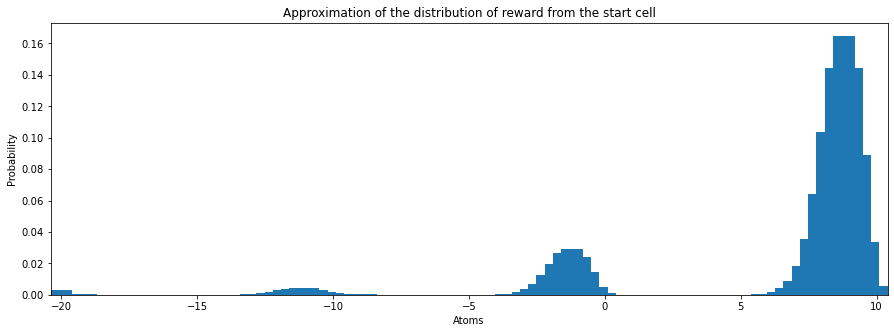
\includegraphics[ width=\textwidth]{figures/personal_work/distrib_mean_99.png}
        \end{subfigure}
            \caption{Behavior on mean optimization $\gamma = 0.99$}
    \end{figure}
    
    \begin{figure}[!ht]
        \centering
        \begin{subfigure}{0.25\textwidth}
            \centering
                \includegraphics[page=4, trim = 40mm 160mm 70mm 45mm, clip, width=0.95\textwidth]{figures/personal_work/policies.pdf}
        \end{subfigure}
        \hfill
        \begin{subfigure}{0.70\textwidth}
            \centering
                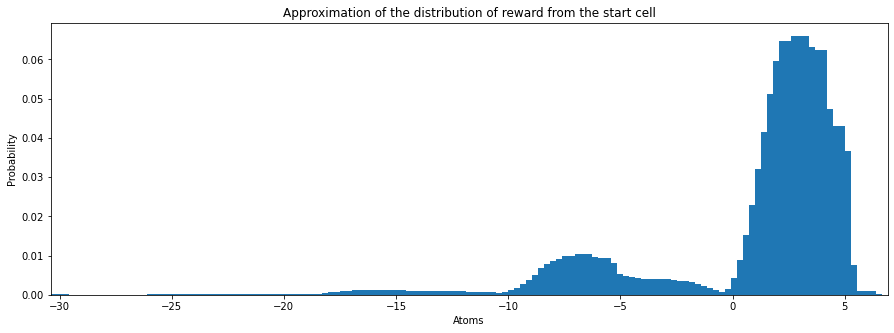
\includegraphics[ width=\textwidth]{figures/personal_work/distrib_mean_9.png}
        \end{subfigure}
            \caption{Behavior on mean optimization, $\gamma = 0.9$}
    \end{figure}
\end{frame}

\begin{frame}{Median case}
    No convergence:

    \begin{figure}[!ht]
        \centering
        \begin{subfigure}{0.24\textwidth}
            \centering
                \includegraphics[page=8, trim = 40mm 160mm 70mm 45mm, clip, width=0.95\textwidth]{figures/personal_work/policies.pdf}
            \caption{1st output policy}
        \end{subfigure}
        \begin{subfigure}{0.24\textwidth}
            \centering
                \includegraphics[page=8, trim = 40mm 40mm 70mm 165mm, clip, width=0.95\textwidth]{figures/personal_work/policies.pdf}
            \caption{2nd output policy}
        \end{subfigure}
            \centering
        \begin{subfigure}{0.24\textwidth}
            \centering
                \includegraphics[page=9, trim = 40mm 160mm 70mm 45mm, clip, width=0.95\textwidth]{figures/personal_work/policies.pdf}
            \caption{3rd output policy}
        \end{subfigure}
        \begin{subfigure}{0.24\textwidth}
            \centering
                \includegraphics[page=9, trim = 40mm 40mm 70mm 165mm, clip, width=0.95\textwidth]{figures/personal_work/policies.pdf}
            \caption{4th output policy}
        \end{subfigure}
            \caption{Policies output by median optimisation}
    \end{figure}

    Issues with equal medians due to the distribution approximation. The medians were still higher than the mean case.
    
\end{frame}


\begin{frame}{Quantile Case}
    \begin{figure}[!ht]
        \centering
        \begin{subfigure}{0.25\textwidth}
            \centering
                \includegraphics[page=7, trim = 40mm 160mm 70mm 45mm, clip, width=0.95\textwidth]{figures/personal_work/policies.pdf}
            \caption{output policy}
        \end{subfigure}
        \hfill
        \begin{subfigure}{0.70\textwidth}
            \centering
                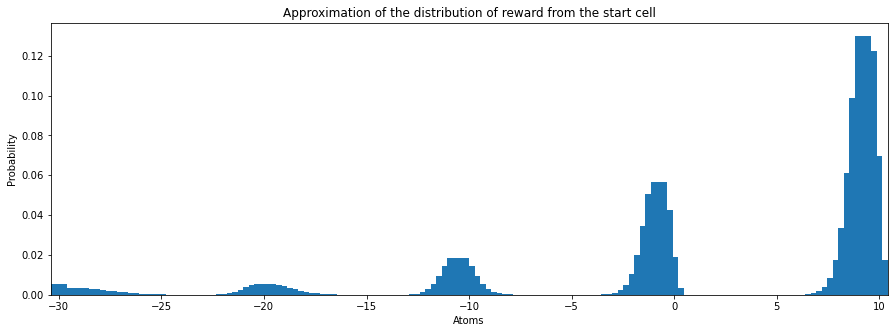
\includegraphics[width=\textwidth]{figures/personal_work/distrib_q80.png}
            \caption{Distribution of return}
        \end{subfigure}
            \caption{Behavior on 0.8 quantile optimazation}
    \end{figure}

    The policy is risky, as expected, and the quantile 0.8 is higher than the mean case.

\end{frame}

\begin{frame}
    \begin{figure}[!ht]
        \centering
        \begin{subfigure}{0.25\textwidth}
            \centering
                \includegraphics[page=6, trim = 40mm 160mm 70mm 45mm, clip, width=0.95\textwidth]{figures/personal_work/policies.pdf}
            \caption{output policy}
        \end{subfigure}
        \hfill
        \begin{subfigure}{0.70\textwidth}
            \centering
                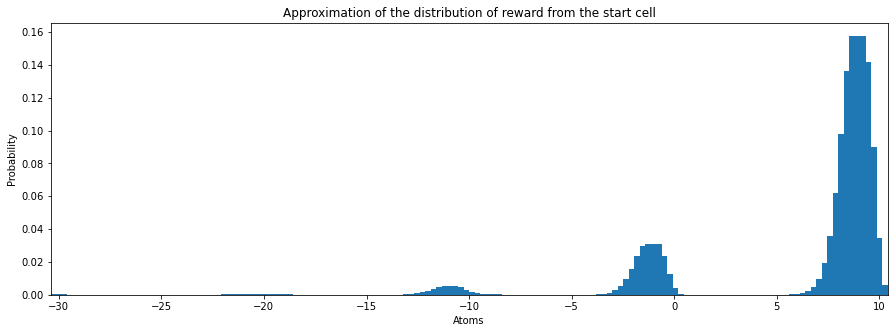
\includegraphics[width=\textwidth]{figures/personal_work/distrib_q20.png}
            \caption{Distribution of return}
        \end{subfigure}
            \caption{Behavior on 0.2 quantile optimazation}
    \end{figure}

    The policy isn’t much safer, and the quantile 0.2 is lower than in the mean case.
\end{frame}

\begin{frame}{About deterministic policies}
    \begin{lemma}
        Let $n \in \NN$, let $0 \leq \lambda_1,\lambda_2,\dots,\lambda_n \leq 1$ such that $\sum_{i = 0}^{n} \lambda_i = 1$, and $\mu_1,\dots, \mu_n $ $n$ distributions. Let $q_\tau$ the quantile function for $\tau \in [0,1]$. We have:
    
        \[ q_\tau \left( \sum_{i=0}^{n} \lambda_i \mu_i\right) \leq \max_{1 \leq i \leq n} q_\tau ( \mu_i) \]
    \end{lemma}
    \begin{Corollary}
        Consider a finite MDP where no state can be visited twice (i.e, without any loops). Consider a state $x \in X$, and $\tau \in [0,1]$. There exist an deterministic policy $\pi^{*}_x$ that optimizes the $\tau$ quantile for state $x$ :
        \[ V_\tau^{\pi^{*}_x(x)} = \max_\pi V_\tau^\pi(x)\]
    \end{Corollary}
\end{frame}

\begin{frame}
    \begin{figure}[!ht]
        \centering
        \begin{tikzpicture} [node distance = 2cm, on grid, auto]
            \node (q1) [state] {$q_1$};
            \node (q2) [state, above right = of q1] {$q_2$};
            \node (q3) [state, right = of q1] {$q_3$};
            \node (q4) [state, below right = of q1] {$q_4$};
            \node (q5) [state, right = of q4] {$q_5$};
            \node (q6) [state, above right = of q5] {$q_6$};
            \node (q7) [state, below right = of q5] {$q_7$};
            \node (q8) [state, right = of q2] {$q_8$};
    
            \path [-stealth, thick]
            (q1) edge node {} (q2)
            (q1) edge node {} (q3)
            (q1) edge node {} (q4)
            (q2) edge node {} (q8)
            (q4) edge node {} (q5)
            (q3) edge node {} (q5)
            (q5) edge node {} (q6)
            (q5) edge node {} (q7);    
    
        \end{tikzpicture}
        \caption{Example of an MDP on which the corollary applies}
    \end{figure}
\end{frame}

\section{Conclusion}

\begin{frame}{Conclusion}
    Main work of the intership:
    \begin{itemize}
        \item Find the bibliography and understand the Distributionnal Framework.
        \item Develop a small librairy to experiment on this distributional framework.
        \item Experiment on it with quantile Optimization, understand behaviors.
        \item Find some counter examples and a little theoretical result.
    \end{itemize}

\bigskip

\textbf{Conclusion of the internship:} Quantile Optimization is hard and the theoretical results are sparse. Some results are promising, but a quantity such as the expectile would be better to optimize on.
\end{frame}

\begin{frame}
    \tiny
    \nocite{*}
    \bibliography{citation} 
\bibliographystyle{ieeetr}
\end{frame}


\end{document}